% !TEX root = ./Thesis.tex

\chapter{Microfluidc Droplet NMR}

The majority of this chapter is work pulsihed in \citep{Hale:2018fv}

\section{Abstract}

In this chapter a system that enables high-resolution NMR spectroscopy of microfluidic droplet
emulsions is discussed. Acquiring NMR spectra of emulsions is complicated by the magnetic
susceptibility mismatches that occur between the phases. In order to overcome these challenges a
2-part solution is needed. Firstly, shim structures are cut into the microfluidic chip in order
to match the PMMA with the continuous phase (cyclohexane). Secondly, an ideal concentration of
chelated $\ce{Eu^{3+}}$ was doped into the dispersed phase (water) in order to match the susceptibility of
the phases. High resolution spectra with linewidths of 3Hz were obtained in the ideal case.
However, a serial dilution experiment that was used to obtain spectra of glucose droplets showed
the highly sensitive dependence of linewidth on Eu concentration.

\section{Introduction}

Droplet microfluidics is the field of microfluidic research that separates samples into discreet droplets by introducing one
immiscible fluid (dispersed fluid) into another (continuous fluid). In this way, samples can be manipulated freely in the lab-on-a-chip (LoC) system,
and problems due to viscous dispersion and cross-contamination
are avoided. In doing so, microdroplets of tuneable size and volume,
typically femto- to nanolitres, are produced at rate reported to be up to 44 kHz \citep{RN115}. Thorsen et al\citep{RN104}
reported one of the first droplet microfluidic devices. In the letter, they show how one can use microfluidic channels to
generate mono-disperse microemulsions by shearing water into a perpendicular flow of oil. By varying the ratio of the pressures
driving the flow of each fluid they produce droplets that range in diameter from 10 $\mu\text{m}$ to 60 $\mu\text{m}$.

Droplets have since emerged as a versatile tool finding wide ranging applications in areas
such as microcapsule synthesis\citep{RN105}, crystal growth\citep{RN106}, chemical reactions
\citep{RN114}, cell/organism encapsulation \citep{RN107,RN108, RN113}, PCR\citep{RN109,
RN110}, and Protein studies\citep{RN111, RN112}. These applications are diverse owing to many
advantages that microfluidic droplets possess: limited cross contamination; high production
rates; large surface area to volume ratio; small reagent volumes; and independent control of
each droplet\citep{RN102}.

Droplet generation can, broadly speaking, be divided into two categories. These are active
and passive generation methods. Active methods are defined as applying additional force to
the device to create droplets such as electric\citep{RN116}, magnetic\citep{RN117} or
centrifugal\citep{RN11} or by modifying intrinsic forces by tuning fluid
velocity\citep{RN58}. Passive methods rely on the inherent instability of the liquid-liquid
interface when mixing two immiscible fluid in order to generate droplets\citep{RN120, RN121,
RN122}. Zhu and wang\citep{RN123} have published an in-depth review of the various methods of
droplet generation as well as the equations that govern them.

In this work, active droplet generation was used in the form of fluid velocity variation. Two
syringe pumps were employed that allowed separate manipulation of flow rates of the dispersed
and continuous fluid. The dispersed and continuous phase are co-flowed to the the droplet
generation point. By using this method, one can control the production rate and size of the
droplets. Droplets of size ~100 $\mu\text{m}$ in diameter and a rate suitable enough to fill
the sample chamber. If the flow is too fast the droplets have a very low residence time and
there is never enough build up to perform an experiment. If, however, the flow is too slow
the droplets that are formed are too big and inconsistent for any kind of reliable
experimentation.

Nuclear magnetic resonance (NMR) as a spectroscopic technique has two chief advantages. It is
non-invasive and non-destructive which makes it ideally placed to study living systems without
destroying them. Indeed, NMR and magnetic resonance imaging (MRI) are both methods actively
employed in metabolomics\citep{RN124}, drug discovery\citep{RN125} and cancer
imaging\citep{RN126}. The nature of NMR means that one can glean quantitative, system
level information in one experiment without the need for chemical tags. In a microfluidic
context, where fluorescence\citep{horrocks2015fast, schlimpert2016fluorescence}, or
mass spec\citep{redman2016characterization,choi2016digital}, are often the methods of choice
for spectroscopy NMR can be used in parallel to these and contribute to a better understanding of the system.

\subsection{Susceptibility}

Magnetic susceptibility, $\chi_V$, is a measure of how much a material will become magnetized in an applied magnetic field. Given by the equation $\mathbf{M} = \chi_V \mathbf{H}$
where $\mathbf{M}$ is the magnetisation of the material and $\mathbf{H}$ is the magnetic field. In \citep{RN118} a derivation of
how the susceptibility can affect the magnetic field around a sample and influence its spectra.

In stationary conditions Ampere’s law gives $\nabla \times \mathbf{H} = 0$ therefore the magnetic field $\mathbf{H}$  can be expressed by scalar magnetic potential $U$ as:
\begin{equation}
\mathbf{H} = -\nabla U
\end{equation}

To describe an object being inserted into a magnetic field we split the potentials as $U = U_{0}  + U_{d}$, where $U_{0} = H_{0}z$ represents the original homogeneous field, and
$\mathbf{H}_d = - \nabla U_{d}$ is the field generated by the magnetic dipoles induced in the inserted object (sometimes referred to as demagnetising field). The magnetic field $H_{0}$, which we assume to be along the z-axis, arises from the superconducting coil

 The macroscopic magnetic induction B is given by:
\begin{equation}
  \mathbf{B} = \mu_{0}(\mathbf{H}+\mathbf{M})
\end{equation}

where $\mu_{0} = 4\pi\times10^{7}~\text{VsAm}^{-1}$ denotes vacuum permeability. With Gauss' law $\nabla \cdot \mathbf{B} = 0$ this becomes:

\begin{equation} \label{eqn1}
  \nabla^{2}U_{d} = \nabla \cdot \mathbf{M}
\end{equation}

We assume the object that the object consists of a number of spatial domains characterised by a
locally constant magnetic susceptibility $\chi_{k}$. The magnetisation therefore, is a piecewise
constant,
\begin{equation}
  \mathbf{M}_{k} = \chi_{k}\mathbf{H}_{k}\mathbf{e}_{z}
\end{equation}

the right hand side vanishes everywhere except at domain boundaries. The magnetic field satisfies the boundary conditions\citep{Jackson:2007uq}

\begin{equation} \label{eqn2}
  (\mathbf{H}_{d2} - \mathbf{H}_{d1}) \times \breve{\mathbf{n}} = 0,
\end{equation}
\begin{equation} \label{eqn3}
    (\mathbf{H}_{d2} - \mathbf{H}_{d1}) \cdot \breve{\mathbf{n}} = H_{0}(\chi_{2} -
    \chi_{1})\mathbf{e}_{z}\cdot\cdot\breve{\mathbf{n}},
\end{equation}

where $\breve{\mathbf{n}}$ denotes the surface norml from material 1 to material 2. Equations \ref{eqn1}, \ref{eqn2} and \ref{eqn3} are formally solved by:

\begin{equation}
  U_{d}(\mathbf{r}) = \frac{H_{0}}{4\pi}\int_{\delta_{12}}\frac{\breve{\mathbf{n}}\cdot\mathbf{e}_{z}(\chi_{2}-\chi_{1})}{\sqrt{(\mathbf{r}-\mathbf{r'})^{2}}}dS,
\end{equation}

where $dS$ is an infinitesimal surface element, and $\mathbf{r'}$ is the interaction variable. If there are more than two materials involved, as there are in droplets, each boundary gives an additive contribution of the same form.

The resonance frequncy observed is proportional to the magnetic induction $\mathbf{B}_ext$
experienced by chemically equivalent nuclei within each domain. This induction is determined
by the outside field $H_{0}$ plus the induced magnetic dipoles of all molecules in the same domain except the one carrying the observed spin.\citep{Levitt:1996tg} In liquids and isotropic solids, the external magnetic induction differs from the macroscopic $\mathbf{B}$ as:

\begin{equation}
  \mathbf{B}_{ext}-\mathbf{B} = \frac{2\mu_{0}\chi_{s}}{3}\mathbf{H}_{0}
\end{equation}

The magnetic induction relvant for the larmour precession of nuclear spins in the sample is therefore

\begin{equation}
  \mathbf{B}_{ext} = \mu_{0}H_{0}(1 + \frac{\chi_{s}}{3})\mathbf{e}_{z} - \mu_{0} \nabla U_{d}
\end{equation}
Since $\chi$ is a piecewise constant, the $\mu_{0} \nabla U_{d}$ term contributes to continuously varying fields
and therefore any line broadening seen in the spectrum, whereas the $\mu_{0}H_{0}(1 + \frac{\chi_{s}}{3})\mathbf{e}_{z}$
produces a bulk magnetic susceptibility shift (BMS) of the resonance line.


Broadly, this allows a classification of most materials as para- ($\chi$>0) or dia- ($\chi$<0) magnetic. Materials used in this work are listed in Table \ref{tab:suscept}

\subsection{Matching susceptibilities in emulsions}


This usually isn’t a problem in microfluidic NMR as usually the materials susceptibilities are matched
in most of our experiments for example the solvent is water and the chip material is PMMA. However,
when the susceptibilities are mismatched, as they are in droplets, this can cause inhomogeneities in
the magnetic field, this shifts the resonances and broadens the lines in the spectra rendering them
useless. For any kind of useful NMR, the magnetic field needs to be very homogeneous with most commercial
superconducting magnets achieving homogeneities of a few parts per billion. Utz and co workers\citep{RN118}
have shown that susceptibility mismatches induced by the doping of $\ce{Eu3+}$ into a solvent can be
compensated for by installing shim structures that contain air around the NMR sensitive region, to produce an
equal and opposite demagnetising field to the one caused by the solution, well
resolved spectra can be taken of glucose dissolved in the mismatched liquid.
\begin{figure}
  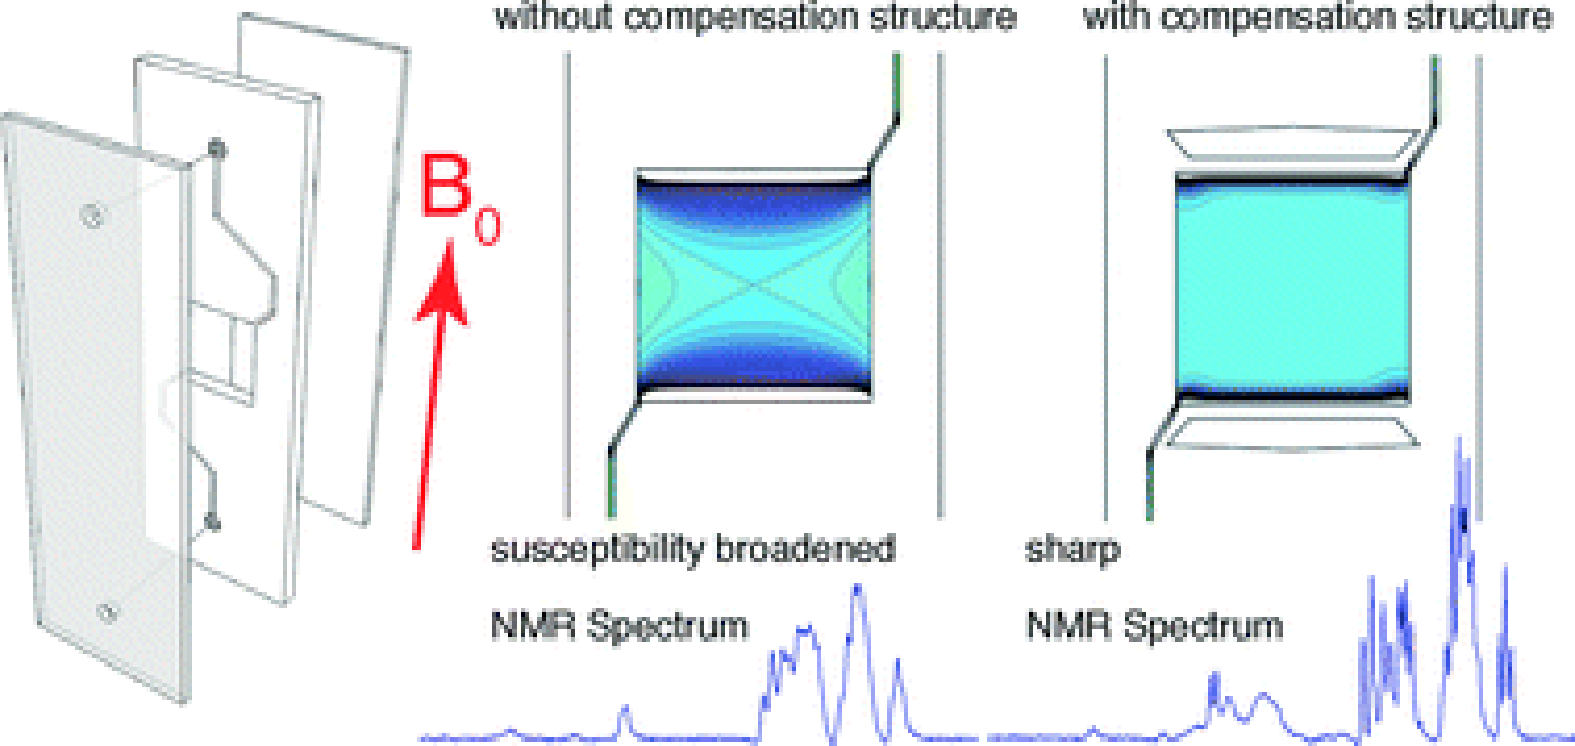
\includegraphics{Utztitle.png}
  \caption{Summary graphic of the work in \citep{RN118}. This shows how the NMR spectrum of glucose
  changes in a suscpetibility mismatched chip but by cuting shimstructures around the sample chamberhigh resolution
  NMR is still possible dspite the mismatches.}
  \label{ShimStructUtz}
\end{figure}

This work, combines both structural shimming and chelated lanthanide doping, to glean high resolution NMR spectroscopy from a microfluidic droplet emulsion. The system, made of a PMMA chip, aqueous dispersed phase and cyclohexane continuous phase. As mentioned the PMMA and water are susceptibility are matched. The cyclohexane, however, is matched to neither. Hence,  for
all materials and solvents to be matched, structural shimming will be employed to match the PMMA to the cyclohexane and a chelated lanthanide $\ce{[Eu(DTPA)]}^{2-}$  will be used to match the water susceptibility.

In emulsions, susceptibility differences between the oil and aqueous phases
lead to similar line broadening\citep{Kuchel:2003ip} NMR spectroscopy is extensively
used to characterise emulsion droplet size distributions using pulsed
field gradient methods\citep{VANDENENDEN:1990ck,FOUREL:1994jv,
Hollingsworth:2004iy,Hindmarsh:2005en,Johns:2009ib,Bernewitz:2011km,Lingwood:2012je}.
These methods do not require spectral resolution of individual
compounds other than the two solvents, and are therefore
unaffected by the susceptibility broadening. By contrast, high-resolution
NMR spectroscopy, with sufficient resolution to distinghuish multiple
compounds present in either of the two phases,
requires careful mitigation of the susceptibility differences. It has also been shown that susceptibility differences can be compensated for in a liquid sample by doping of a chelated lathanide\citep{fabry1983effect}
For example, Lennon \emph{et al.} demonstrated that the susceptibility mismatch between the inside and outside of deoxygenated red blood cells could be
compensated for by doping 3mM of dysprosium tripolyphosphate $\ce[{Dy(PPP)_2}]^{7-}$ into the extracellular fluid\citep{lennon1994hemoglobin}

\begin{figure}
  \begin{center}
    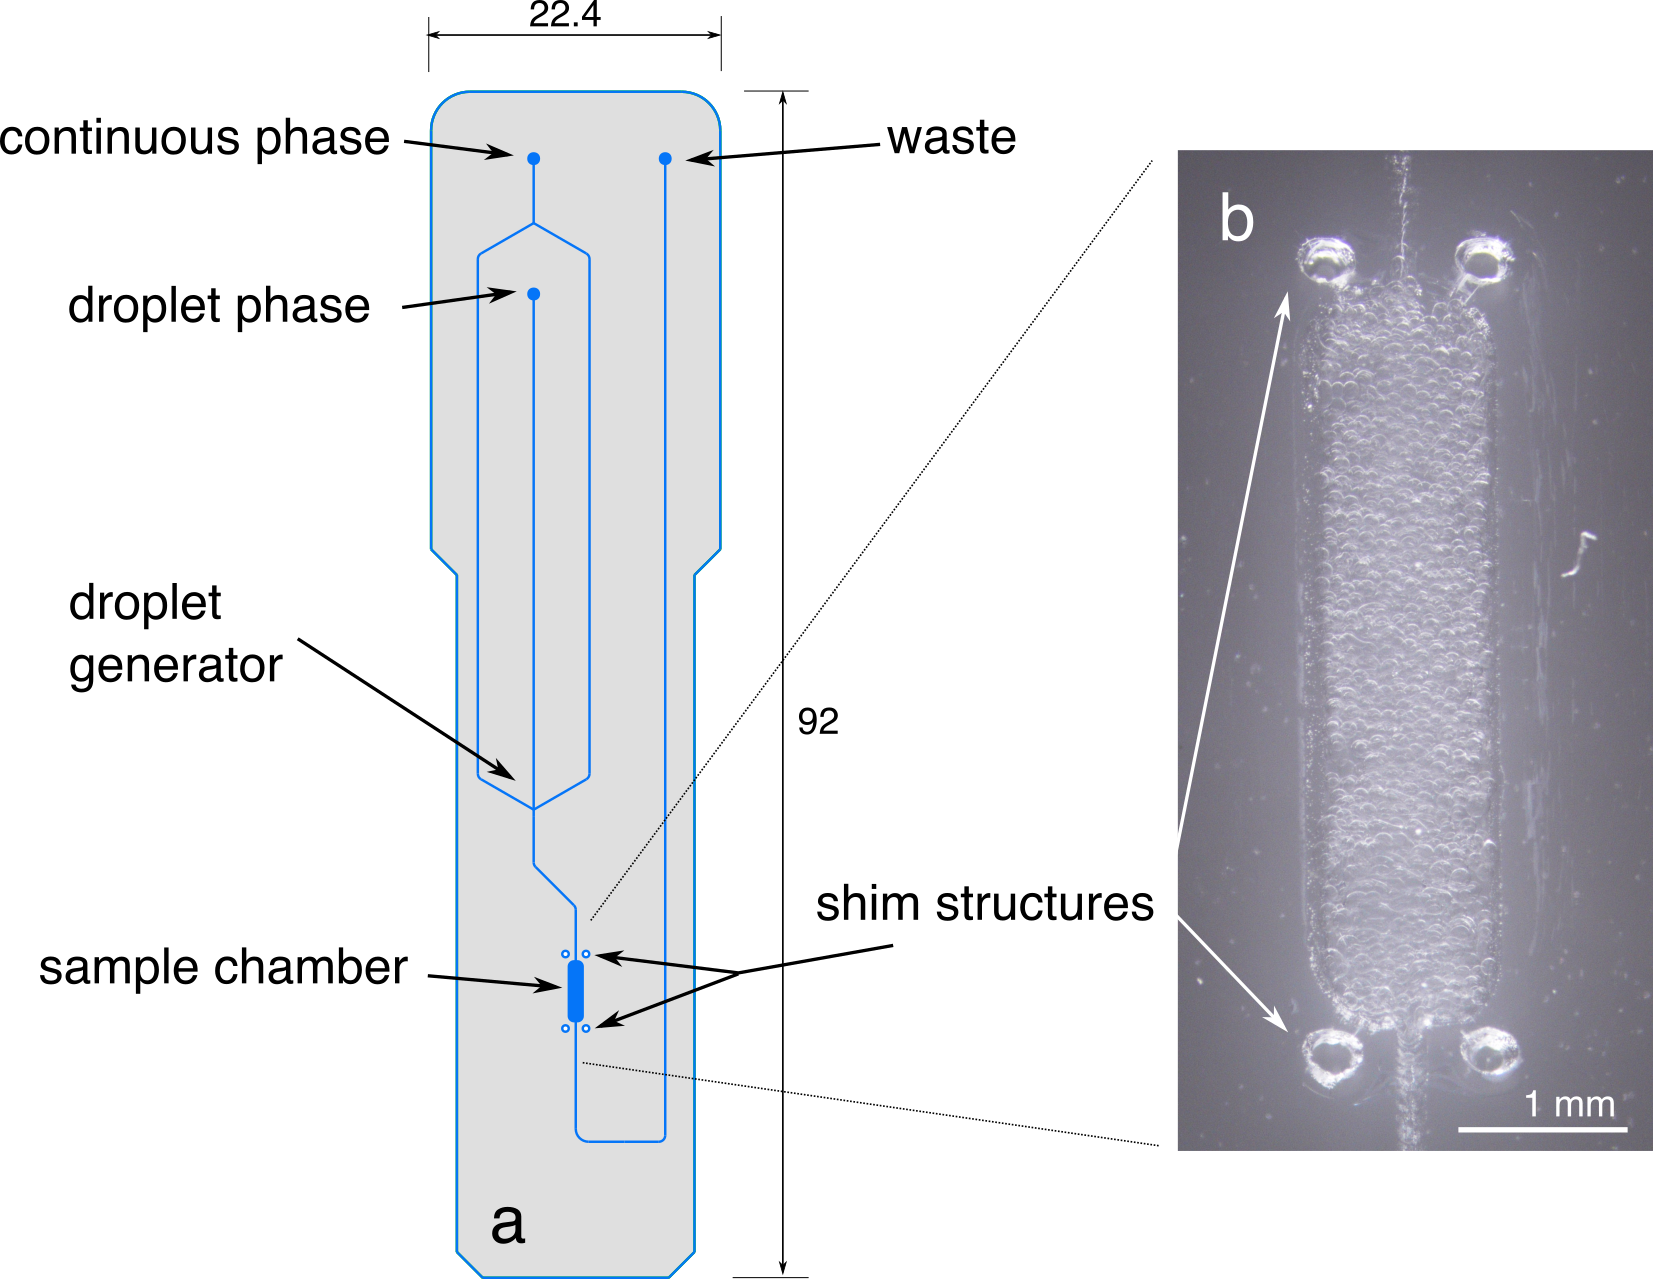
\includegraphics[width=0.8\columnwidth]{mu1y11-dnmr-fi-180421-chip-schematic}
  \end{center}
  \caption{Droplet chip design (left) and detail micrograph of the sample chamber
  area filled with droplets (right). Some droplets are also visible in the
  entrance and exit channels.}
  \label{fig:chip-design}
\end{figure}

In this work, the possibility to obtain high-resolution NMR spectra from
small volumes of droplet emulsions on a chip is explored.
Integration of high-resolution NMR spectroscopy with microfluidic systems is
challenging for a number of reasons.
On the one hand, small sample volumes place stringent demands on detector
sensitivity\citep{Badilita:2011td,Zalesskiy:2014hi}
This has recently been addressed with the design of
highly efficient planar NMR microcoils\citep{Spengler:2016km} and
transmission line resonators\citep{Finch:2016gv}
Another challenge is the preservation of high spectral
resolution, which depends on a highly homogeneous magnetic field
over the sample volume. Differences in magnetic susceptibility
between the materials used for the microfluidic chip
and the sample fluid, as well as the materials and geometry
of the probe assembly, lead to a demagnetising field
that varies continously over the sample volume. Typical diamagnetic
volume susceptibilties range from about
$-11$~ppm to about $-5$~ppm (in SI units);\citep{Kuchel:2003ip,Durrant:2003kv}
differences of the order of several ppm are therefore commonplace.
Unmanaged, they lead to
broadening of NMR spectral lines over a ppm or more, which
corresponds to a severe loss of resolution in $\ce{^1H}$ liquid
state NMR.

Managing susceptibility differences for an emulsion of droplets on a
microfluidic chip adds additional complexity, since three different materials
are now involved: the chip, the continuous phase, and the droplet phase,
all with different susceptibilities.
This can be mitigated in a two-step approach,
which is based on the observation that most organic solvents in use
as continuous phases for droplet microfluidics are less diamagnetic than
water.
First, the susceptibility difference between the chip and the continuous phase
are compensated by shimming structures that are added to the
chip design. Then, the susceptibility of the aqueous droplet phase is matched
to that of the continuous phase by adding a paramagnetic solute.

It should be noted that in principle, the same effect could be achieved if
a diamagnetic dopant could be added to the continuous phase. However, while paramagnetic
dopants are easily available in the form of transition metal ions, no
effective diamagnetic dopants exist in the literature.

$\ce{Eu^{3+}}$ complexes are paramagnetic, and are frequently used as
shift agents in NMR spectroscopy. Unlike other lanthanide ions such
as $\ce{Gd^{3+}}$ or $\ce{Ho^{3+}}$, which are powerful nuclear relaxation
agents, $\ce{Eu^{3+}}$ has only a minimal
effect on nuclear magnetic relaxation due to its extremely
short electron spin-lattice relaxation time\citep{Peters:1996bj} Addition of
millimolar quantities of $\ce{Eu^{3+}}$ to aqueous solutions
therefore does not cause significant relaxation line broadening, but changes
the bulk magnetic susceptibility of the solution proportionally
to the $\ce{Eu^{3+}}$ concentration. It is therefore possible
to adjust the susceptibility difference in a droplet emulsion
by adding a $\ce{Eu^{3+}}$ complex that selectively dissolves in (or at least
strongly partitions to) the aqueous phase.


\begin{table}
\begin{center}
    \caption{Bulk magnetic susceptibilities}
    \label{tab:suscept}
    \begin{tabular}{lcc}\hline\hline
      \emph{Compound} & $\chi_V/10^{-6}$ (SI) & Ref \\ \hline
      water           & $-9.05$               &    \citep{Rumble:2017tp}  \\
      cyclohexane     & $-7.640$              &    \citep{Rumble:2017tp} \\
      PMMA            & $-9.01$               &    \citep{Wapler:2014es}\\
      Air             & $+0.36$               &    \citep{Bakker:2006eea} \\ \hline\hline
    \end{tabular}
\end{center}
\end{table}



\begin{figure}
  \begin{center}
    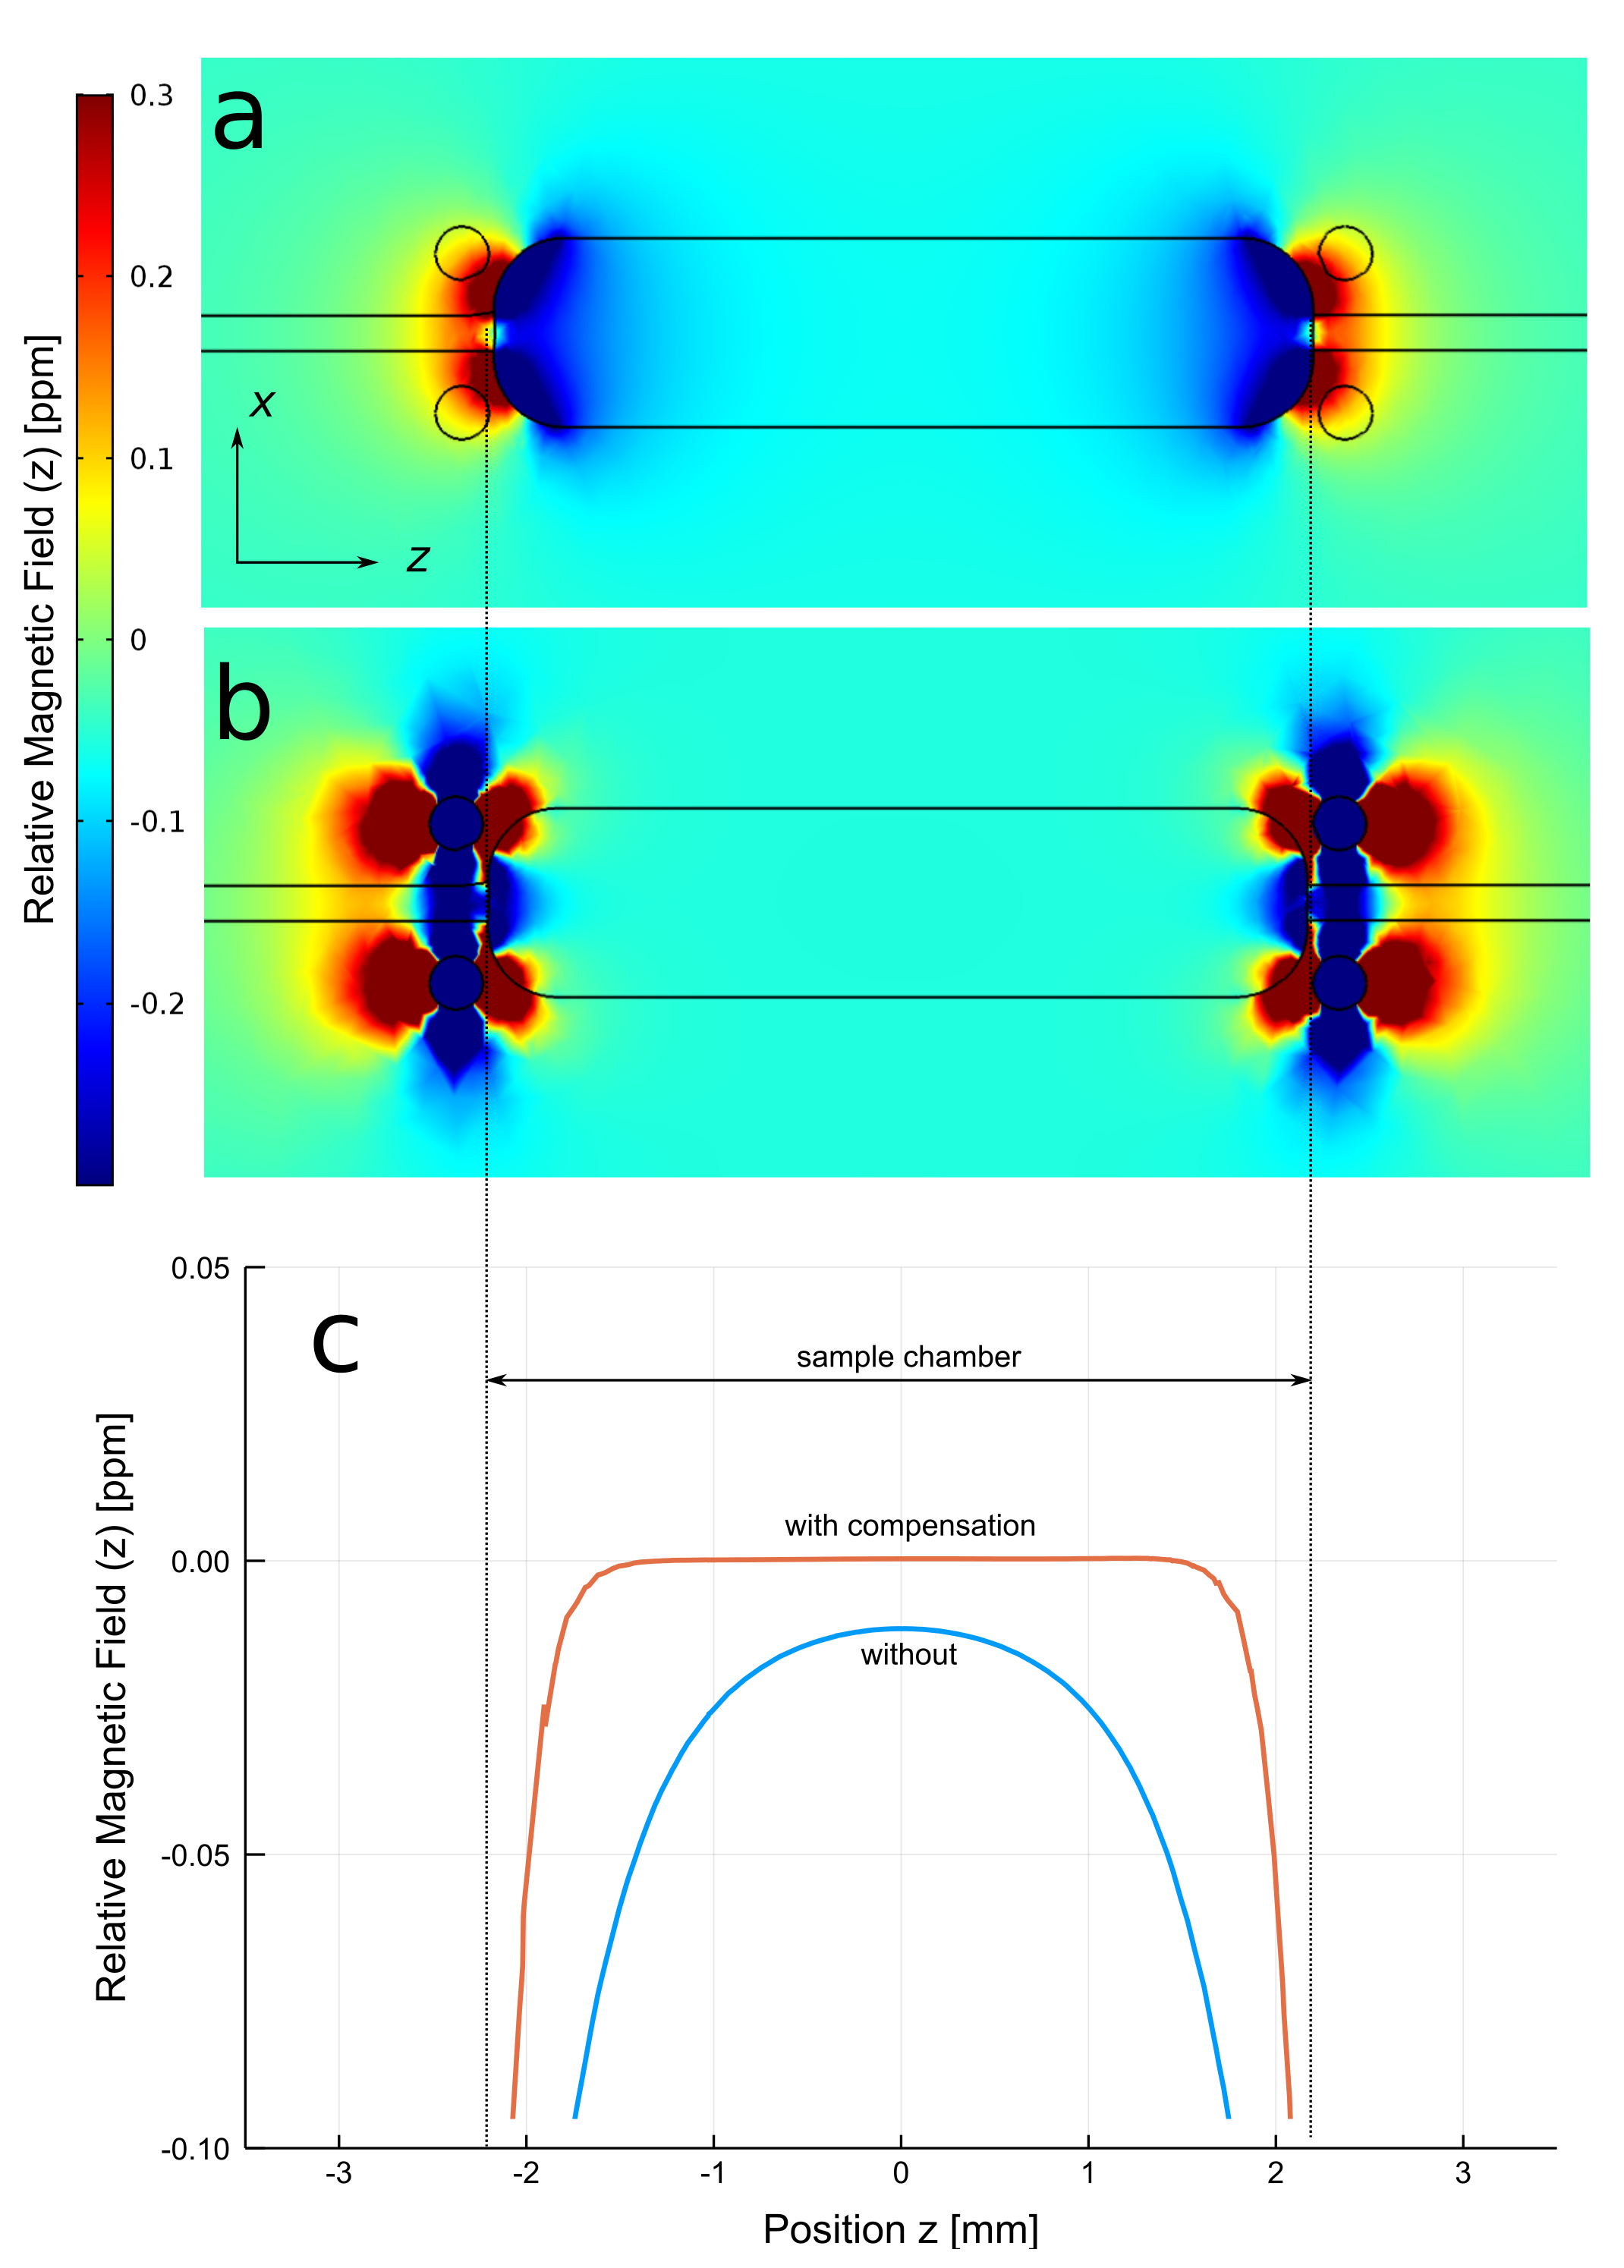
\includegraphics[width=0.8\columnwidth]{mu1y11-dnmr-fi-180421-chip-FEM.png}
  \end{center}
  \caption{A: Finite element simulation of relative magnetic field distribution in an uncompensated chip (circular structures filled with PMMA) filled with cyclohexane
      and B: a compensated chip filled with cyclohexane; C: a linear plot of relative magnetic field along the z-axis through the middle of the sample chamber.
    }
  \label{fig:FEM-chip}
\end{figure}


\begin{figure}
  \begin{center}
    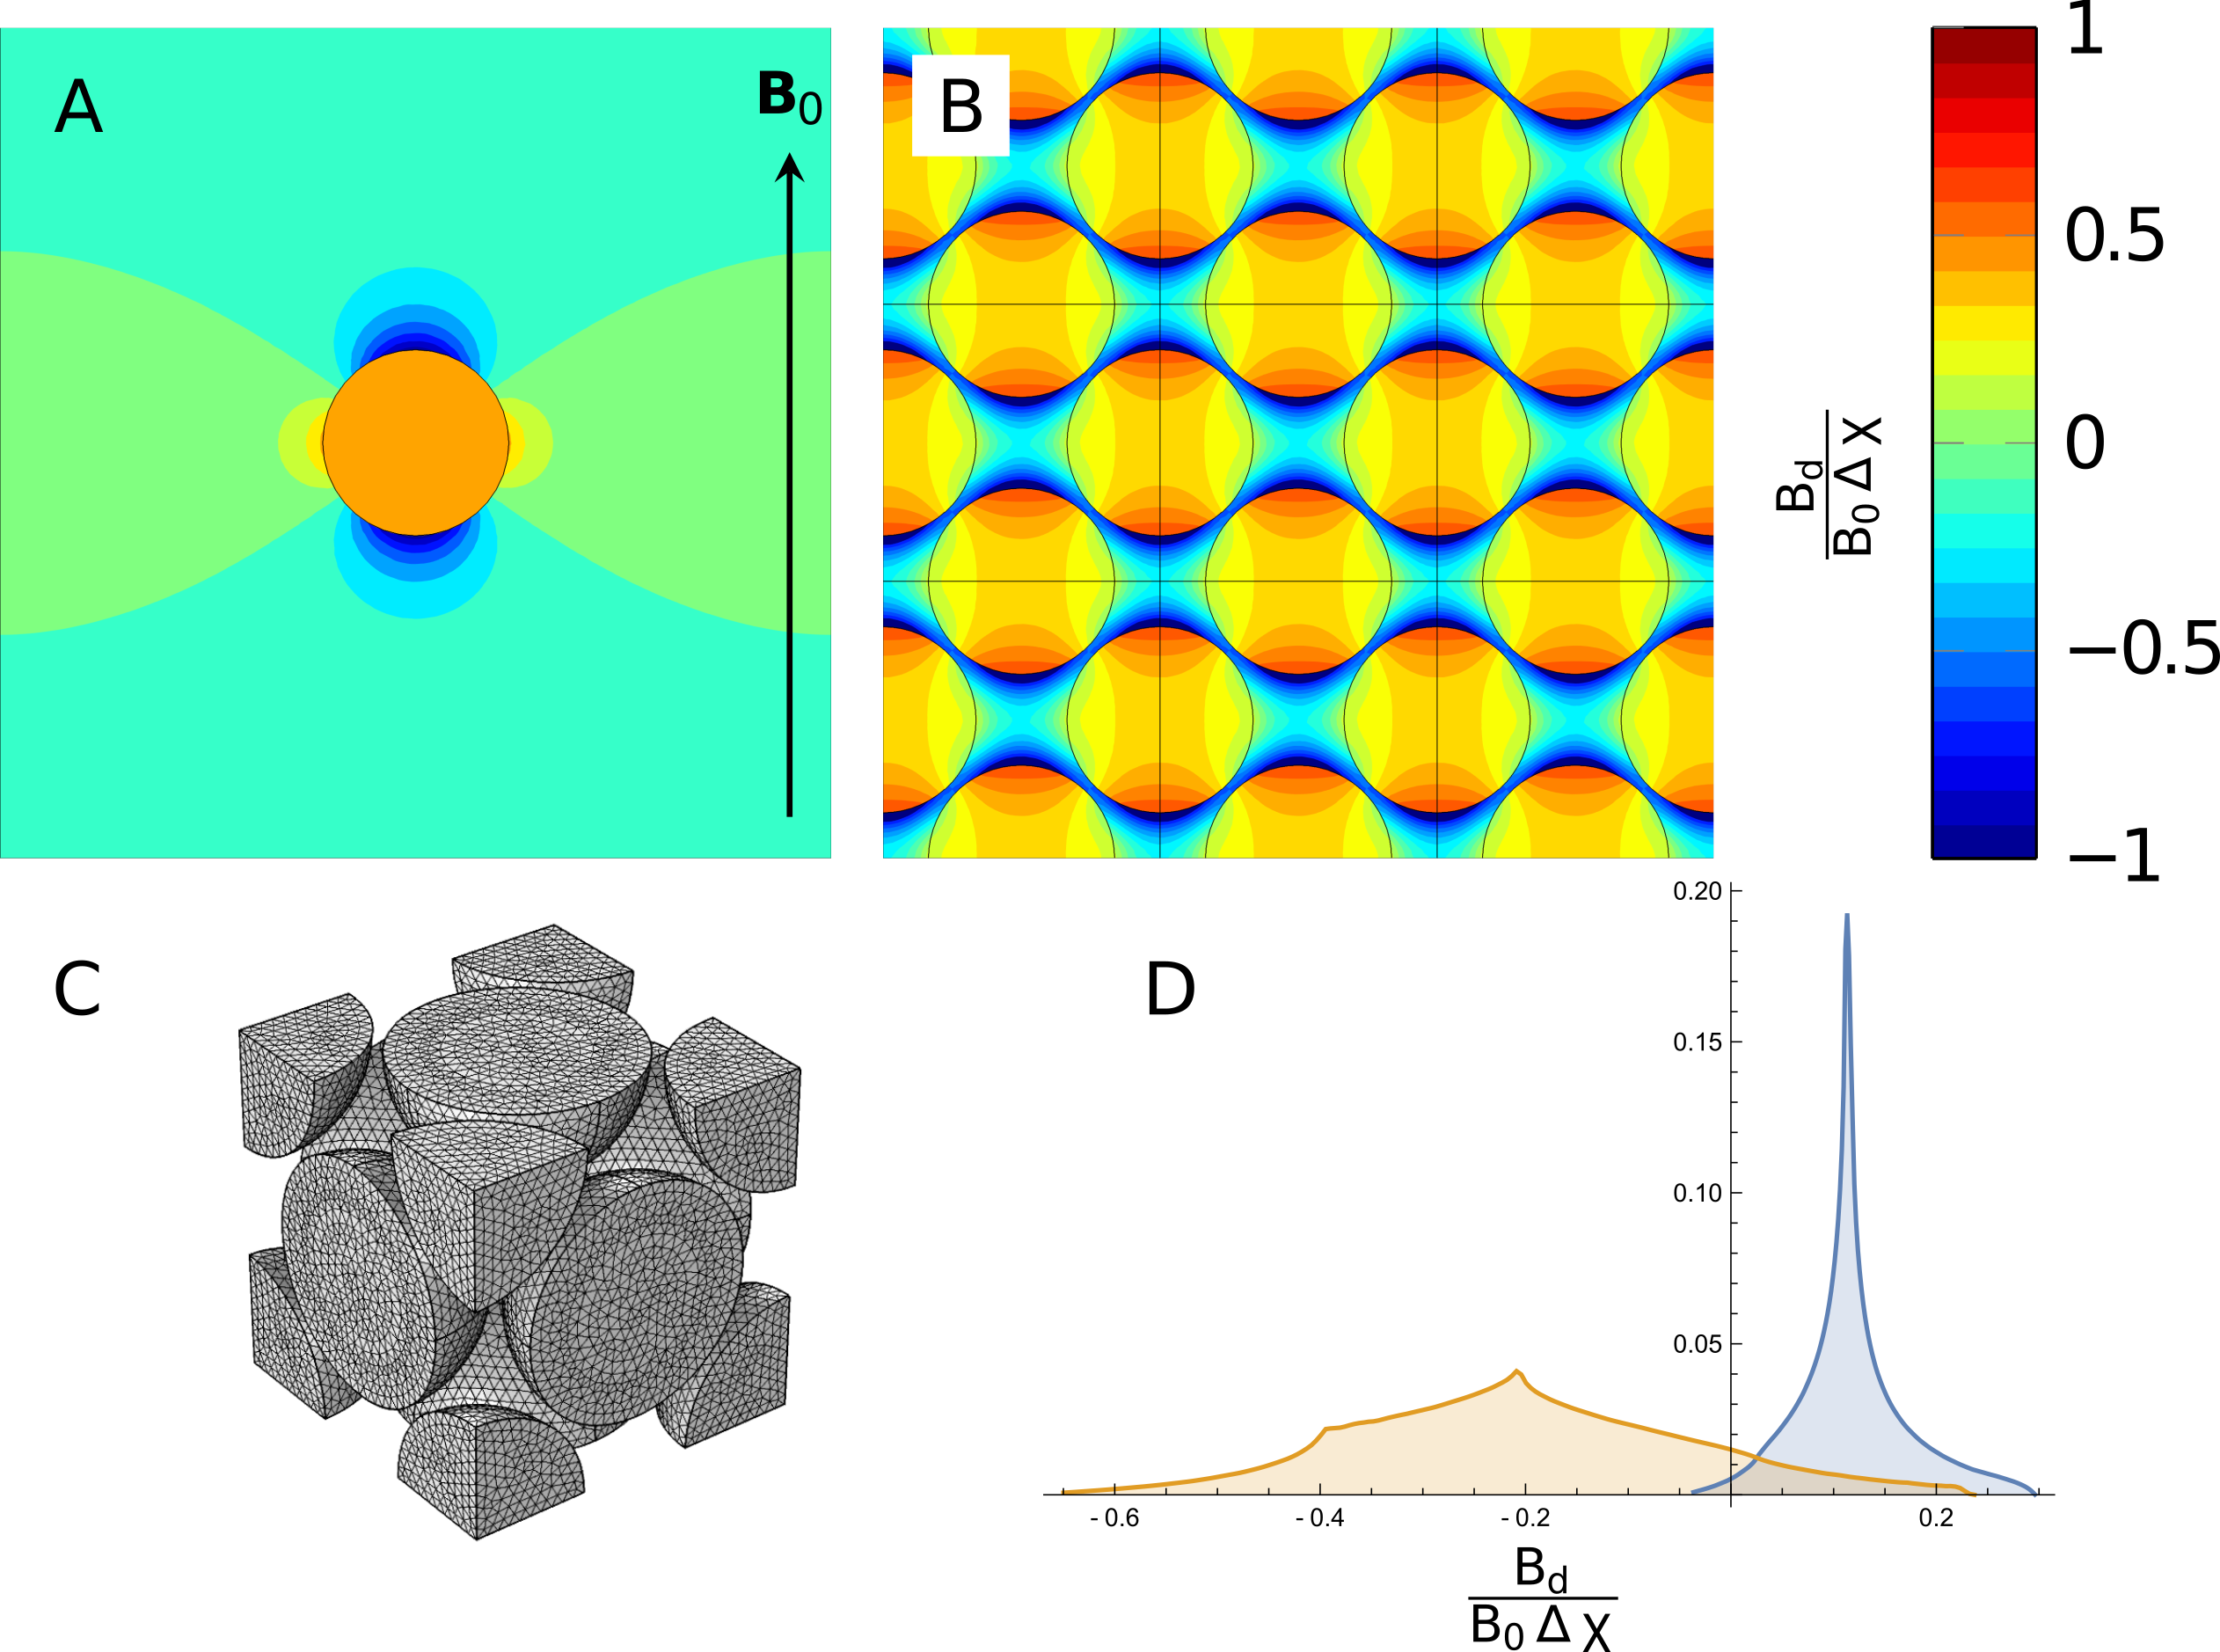
\includegraphics[width=\columnwidth]{mu1y11-dnmr-fi-180629-fcc-simulated}
  \end{center}
  \caption{A: Finite element simulation of magnetic field distribution in droplets.
      $z$-component of the reduced magnetic field $H_\text{red}$ in an isolated spherical droplet
      and B: in a face-centred cubic arrangment of droplets; C: FEM mesh used
      to calculate the result shown in B; D: histograms of the $z$-component
      of the reduced magnetic field in the continuous (orange) and in the droplet (blue) phase
      in the FCC arrangement.
    }
  \label{fig:FEM-fcc}
\end{figure}


In the present work, the diethyl-triamine pentaacetate (DTPA) complex
of $\ce{Eu^{3+}}$, $\ce{Eu[DTPA]^{2-}}$ is used. As an ion species, it is readily soluble
in aqueous media, while exhibiting only negilgible solubility in apolar organic
solvents. Microfluidic chips are fabricated from poly methyl methacrylate (PMMA).
By a fortunate coincidence, the suceptibilities of PMMA and
water are very close to
each other (Table \ref{tab:suscept}).  NMR lines
in microfluidic devices made from PMMA are therefore narrow
if  aqueous samples are used, provided that the boundaries of the chip and the environment
are either aligned with the external magnetic field, or are kept sufficiently
remote from the detection area. By contrast, most organic solvents are
considerably less diamagnetic than water, as exemplified by the
case of cyclohexane, which has been used in the present study.


In the remainder of this chapter,
finite element calculations (Should I add something about M. Utz perfomring these?) are used to estimate
the NMR line widths expected in a droplet emulsion
depending on the susceptibility mismatch.
The results are then compared to experimental
line widths obtained with varying concentrations
of $\ce{Eu[DTPA]^{2-}}$ in the aqueous phase. Finally,
 narrow NMR lines are obtained by
combining structural shimming\citep{Ryan:2014hl} with
susceptibility matching, and demonstrate that this
approach can be used to obtain a high resolution of glucose contained within the compensated droplets.
The chip used in this work is shown in \fig{fig:chip-design}. It consists of a sample
chamber in the centre of the chip, which is designed to line up with
the sensitive area of a transmission-line
micro-NMR detector,\citep{Finch:2016gv} and a convergent flow droplet
generator. The aqueous phase and the continuous
phase are fed into the two ports at the top. Droplets are
formed and transported downstream into the sample chamber.
 The chamber is surrounded by four shim structures, which are circular
 shaped cutouts filled with air. They have been designed to compensate
 for the difference in susceptibility between the chip material (PMMA)
 and the oil phase (cyclohexane) as shown in \fig{fig:FEM-chip}. The operation of the chip is shown
 on the right side of \fig{fig:chip-design}; droplets of about 100~$\mu$m diameter are formed and
 fill the sample chamber.



\begin{figure}
  \begin{center}
    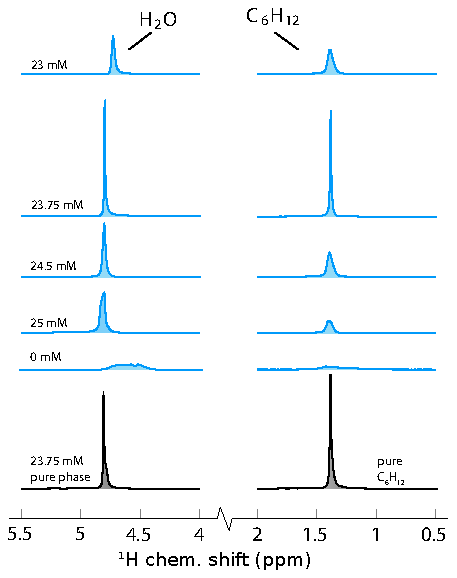
\includegraphics[width=0.7\columnwidth]{normalised-new-droplet-spectra}
  \end{center}
  \caption{$^1$H NMR line shapes of water (left) and cyclohexane (right) of a
  water in cyclohexane emulsion as a function of $\ce{Eu[DTPA]^{2-}}$ concentration
  in the aqueous phase normalised to the sharpest peak. The spectra given in black are the pure phase spectra produced by the same chip.
  }
  \label{fig:droplet-spectra}
\end{figure}


\begin{figure}
  \begin{center}
    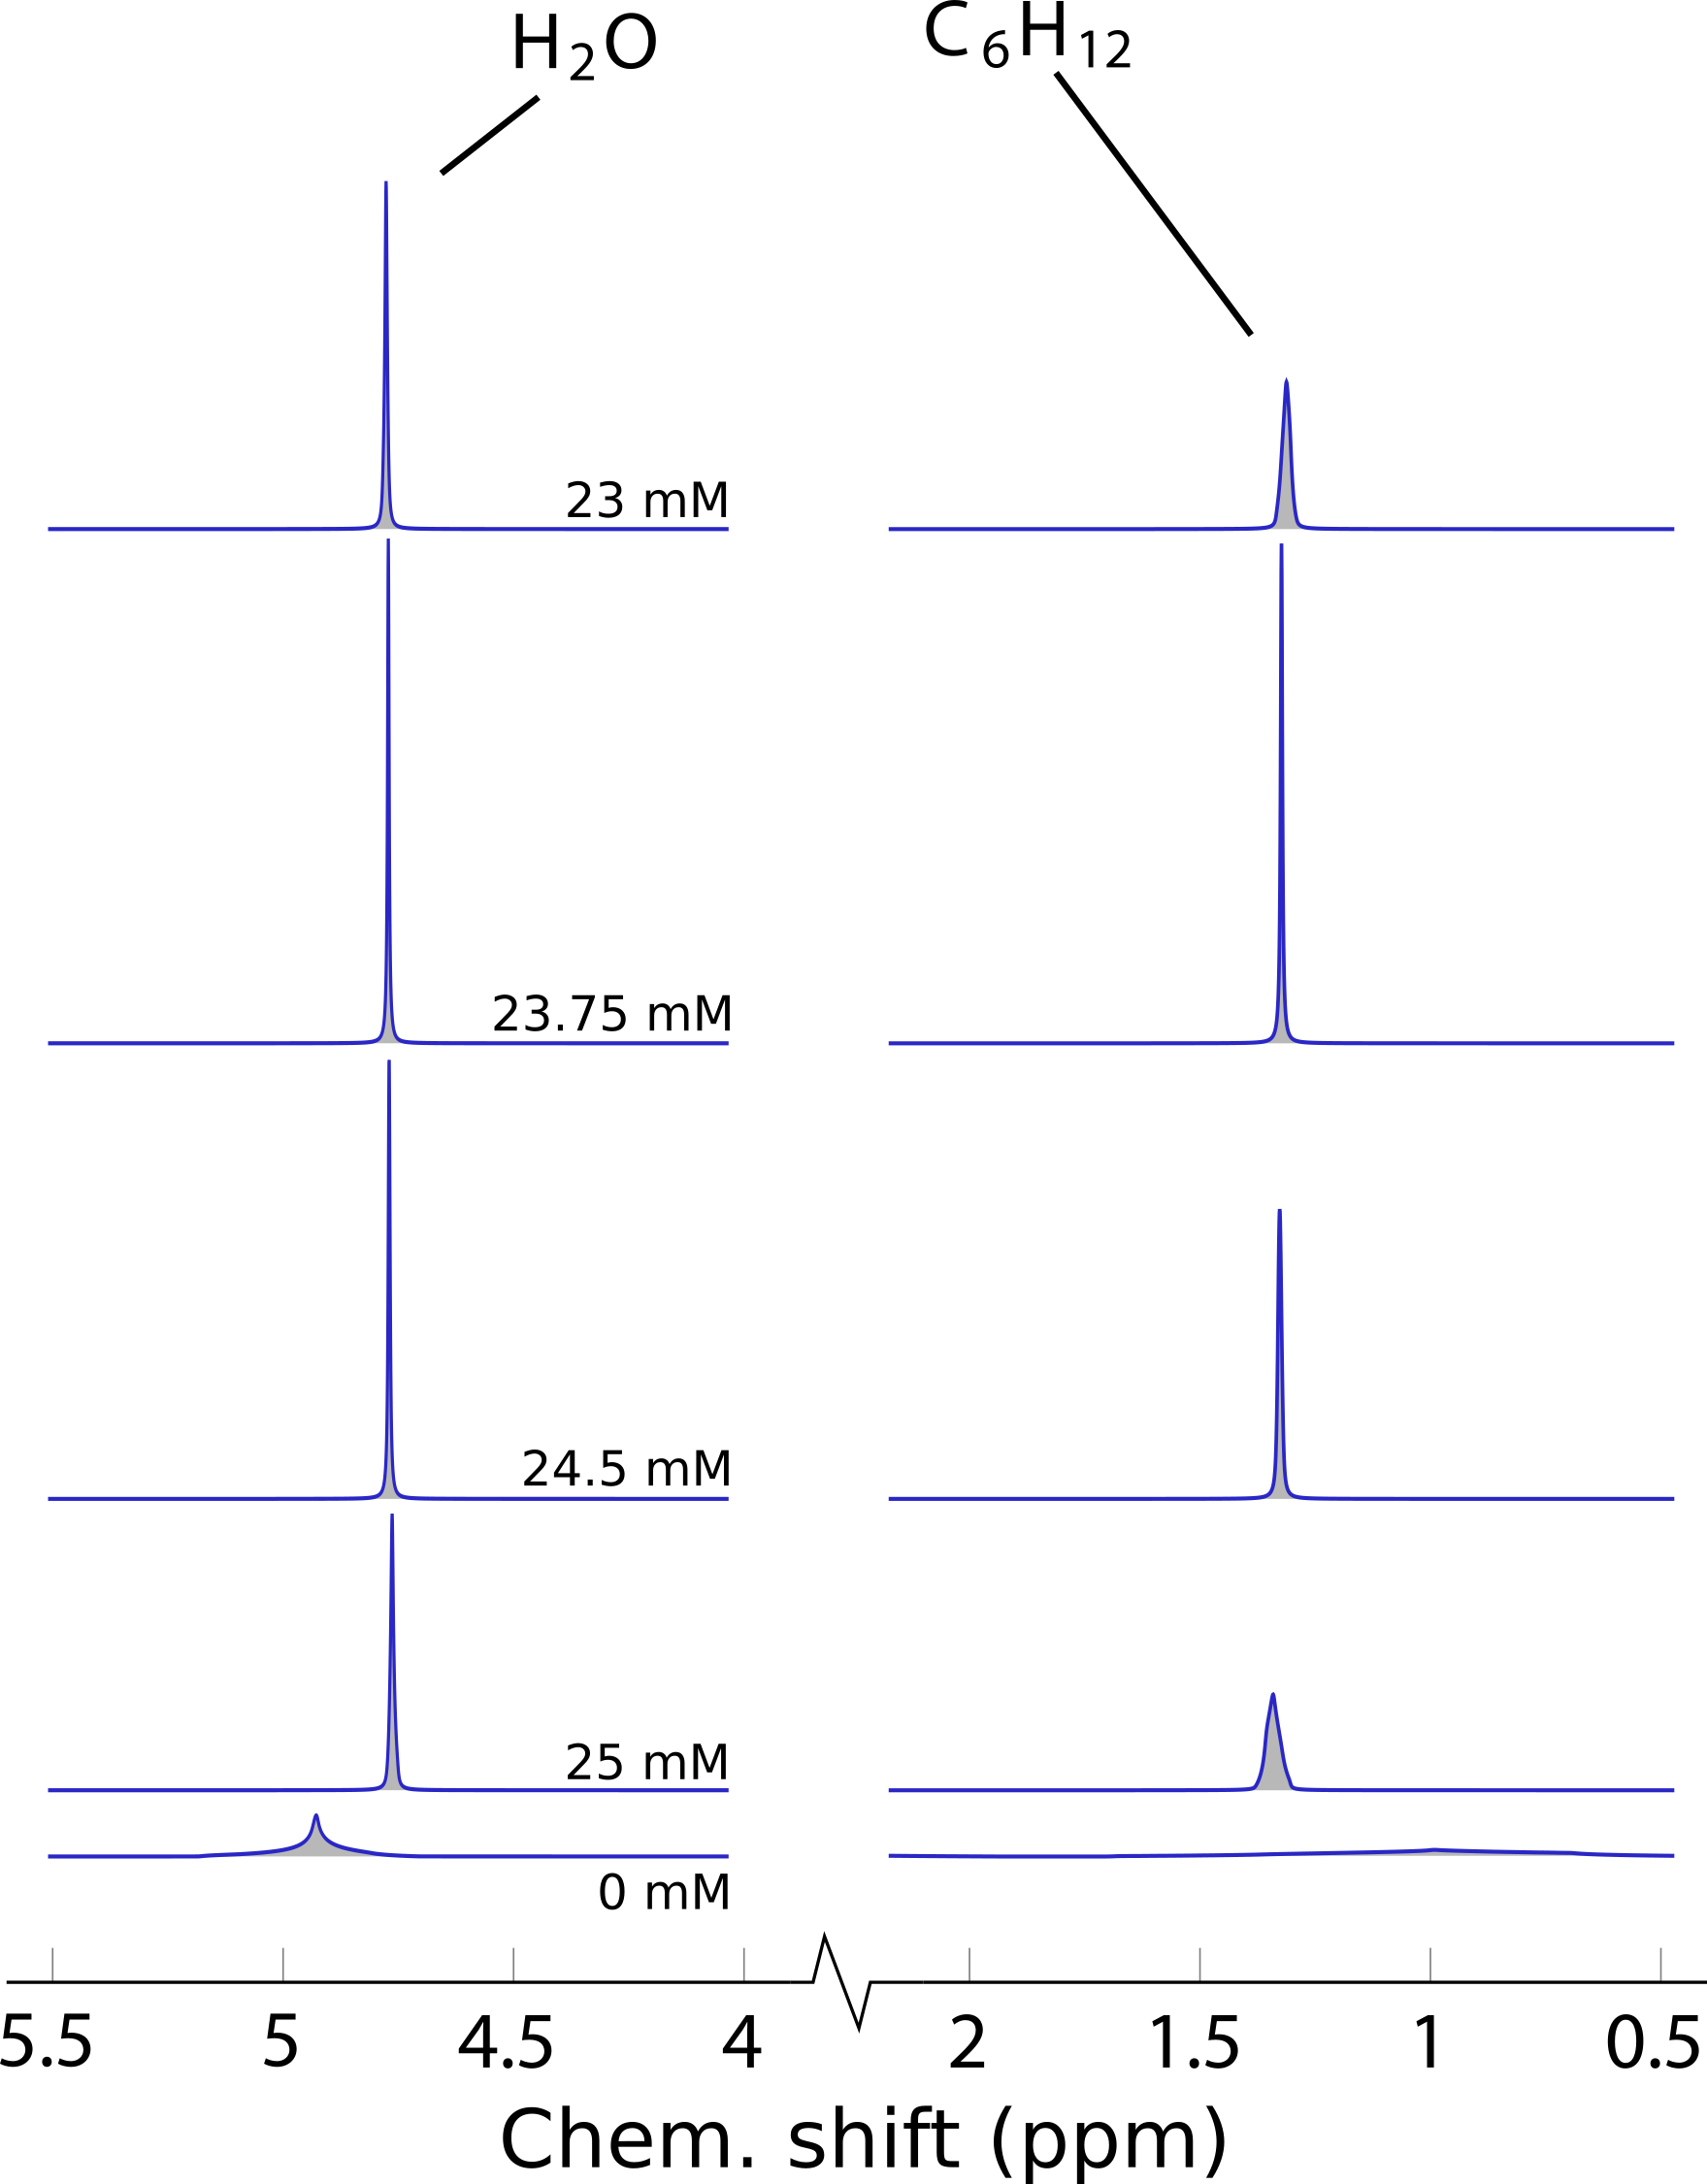
\includegraphics[width=0.7\columnwidth]{mu1y11-dnmr-fi-180622-simulated.png}
  \end{center}
  \caption{Predicted $^1$H NMR line shapes of water (left) and cyclohexane (right) of a
  water in cyclohexane emulsion as a function of $\ce{Eu[DTPA]^{2-}}$ concentration
  in the aqueous phase.
  }
  \label{fig:predicted-spectra}
\end{figure}




\section{Materials and Methods}

Microfluidic chips of the design shown in \fig{fig:chip-design}
were fabricated from PMMA sheet material by
laser cutting, and subsequent bonding of layers with a plasticiser
under heat and pressure\citep{Yilmaz:2016fx} The chips consist of a
top and bottom layer of 200~$\mu$m thickness each, and a middle layer of
500~$\mu$m. Fluid channels upstream from the flow-focussing droplet
generator were scored into the middle layer at low laser power to a depth
of about 100~$\mu$m. Downstream from the droplet generator, the channels and
the sample chamber were cut through the 500 $\mu$m middle layer by increased
laser power, as were the shimming structures. The chips were connected to
a pair of Cole-Palmer 200-CE syringe pumps for droplet generation.
A flow rate of 20~$\mu$l/min was typically used for the continuous
phase and 4~$\mu$l/min for the aqueous droplet phase.
The continuous phase consisted of cyclohexane (Sigma-Aldrich)
with 0.5\% w/v of span-65 (sorbitan
tristearate, Sigma-Aldrich) as a surfactant to ensure droplet stability.
The cyclohexane/span solution was kept in a water bath at 30$^\circ$C
for at least 2h to ensure complete dissolution of the span.
Prior to use, all solutions were left to equilibrate at a controlled room temperature
of 25$^\circ$C for at least 4h.
Steady state conditions were ensured by letting the droplet generation run until
the volume inside the chip had been exchanged at least five times. The
chip was then disconnected from the syringe pumps, and the connection
points sealed prior to insertion of the chip into the NMR probe.

NMR measurements were carried out on a Bruker AVANCE III
spectrometer equipped with an Oxford wide bore magnet operating at 7.05 Tesla,
corresponding to a $\ce{^1H}$ Larmor frequency of 300 MHz. A home-built NMR probe
based on a transmission-line detector was used\citep{Finch:2016gv}
It accommodates microfluidic chips of the shape shown in \fig{fig:chip-design}.
In the present work, the probe was doubly
tuned to allow irradiation both at 300 MHz for $\ce{^1H}$ and at 75 MHz for
$\ce{^{13}C}$. Details of the electronic and mechanical design of the
probe are given in Ref.~\citep{Finch:2017vb}.

NMR spectra were obtained at an RF nutation frequency of 66 kHz for
$\ce{^1H}$, corresponding to 90 degree pulse length of
3.8 $\mu$s. Shimming of the sample was first performed on a sample of pure cyclohexane
in an identical chip, these resulting values were used throughout all subsequent experiments with
minor adjustments being made to linear shims (X,Y,Z) before each experiment to minimise line width. NMR spectra were acquired using Bruker spectrometer software (TopSpin 2.0),
and were processed using home-built scripts written in \textit{Julia}.\citep{Bezanson:2017gd}
20~mM of 4,4-Dimethyl-4-silapentane-1-sulfonic acid (DSS, Sigma Aldrich) was added to the aqueous phase
as a chemical shift standard.

MRI gradient echo images of the sample chamber were obtained using ParaVision software and the fast low-angle shot (FLASH) pulse program. Flip angles of 30$^\circ$ were employed as well as a repetition time of 600 ms; 8 scans were averaged for each image. Two images were acquired for each field map at echo times of 6 and 10ms, respectively. The data was processed using home built software in \textit{Mathematica}.

$\ce{Eu[DTPA]^{2-}}$ solutions were prepared  from a $82.2\pm0.25$~mM
stock solution, which was prepared by adding 1 g of $\ce{EuCl_3}$
(Sigma Aldrich) to a 50 mL volumetric flask. Separately,
3.93 g of diethylenetriaminepentaacetic acid (DTPA, Sigma Aldrich)
and 1.99 g of NaOH (Fischer) were dissolved in 100 mL deionised (DI) water (Sigma Aldrich) .
An equimolar amount of the DTPA solution was added to the $\ce{EuCl_3}$ solution. The pH of this solution was then adjusted by addition of 2M NaOH solution dropwise until a neutral pH was attained.
This was then topped up to 50 mL using DI water.

Finite element calculations of field distributions in emulsions
 were carried out using COMSOL Multiphysics with the "magnetic fields, no currents" (mfnc) physics module.
Optimisation of the shim structures was done with COMSOL Multiphysics\citep{comsolmp} Starting from a SolidWorks model
of the chip design, which was also used as a basis for production of the devices using
a laser cutter, a finite element model was assembled and meshed. The shim structures consist
of four symmetrically arranged circular holes through the middle layer of the three-layered
devices. The positions and the diameters of these
holes were optimised using a Nelder-Mead simplex algorithm. At each iteration, the magnetic
field distribution inside the sample chamber was calculated using the mfnc physics module.
The square norm of the second derivative of the $z$-component of the magnetic field was integrated
over the volume of the sample chamber, and was used as optimisation target.

\begin{figure}
  \begin{center}
    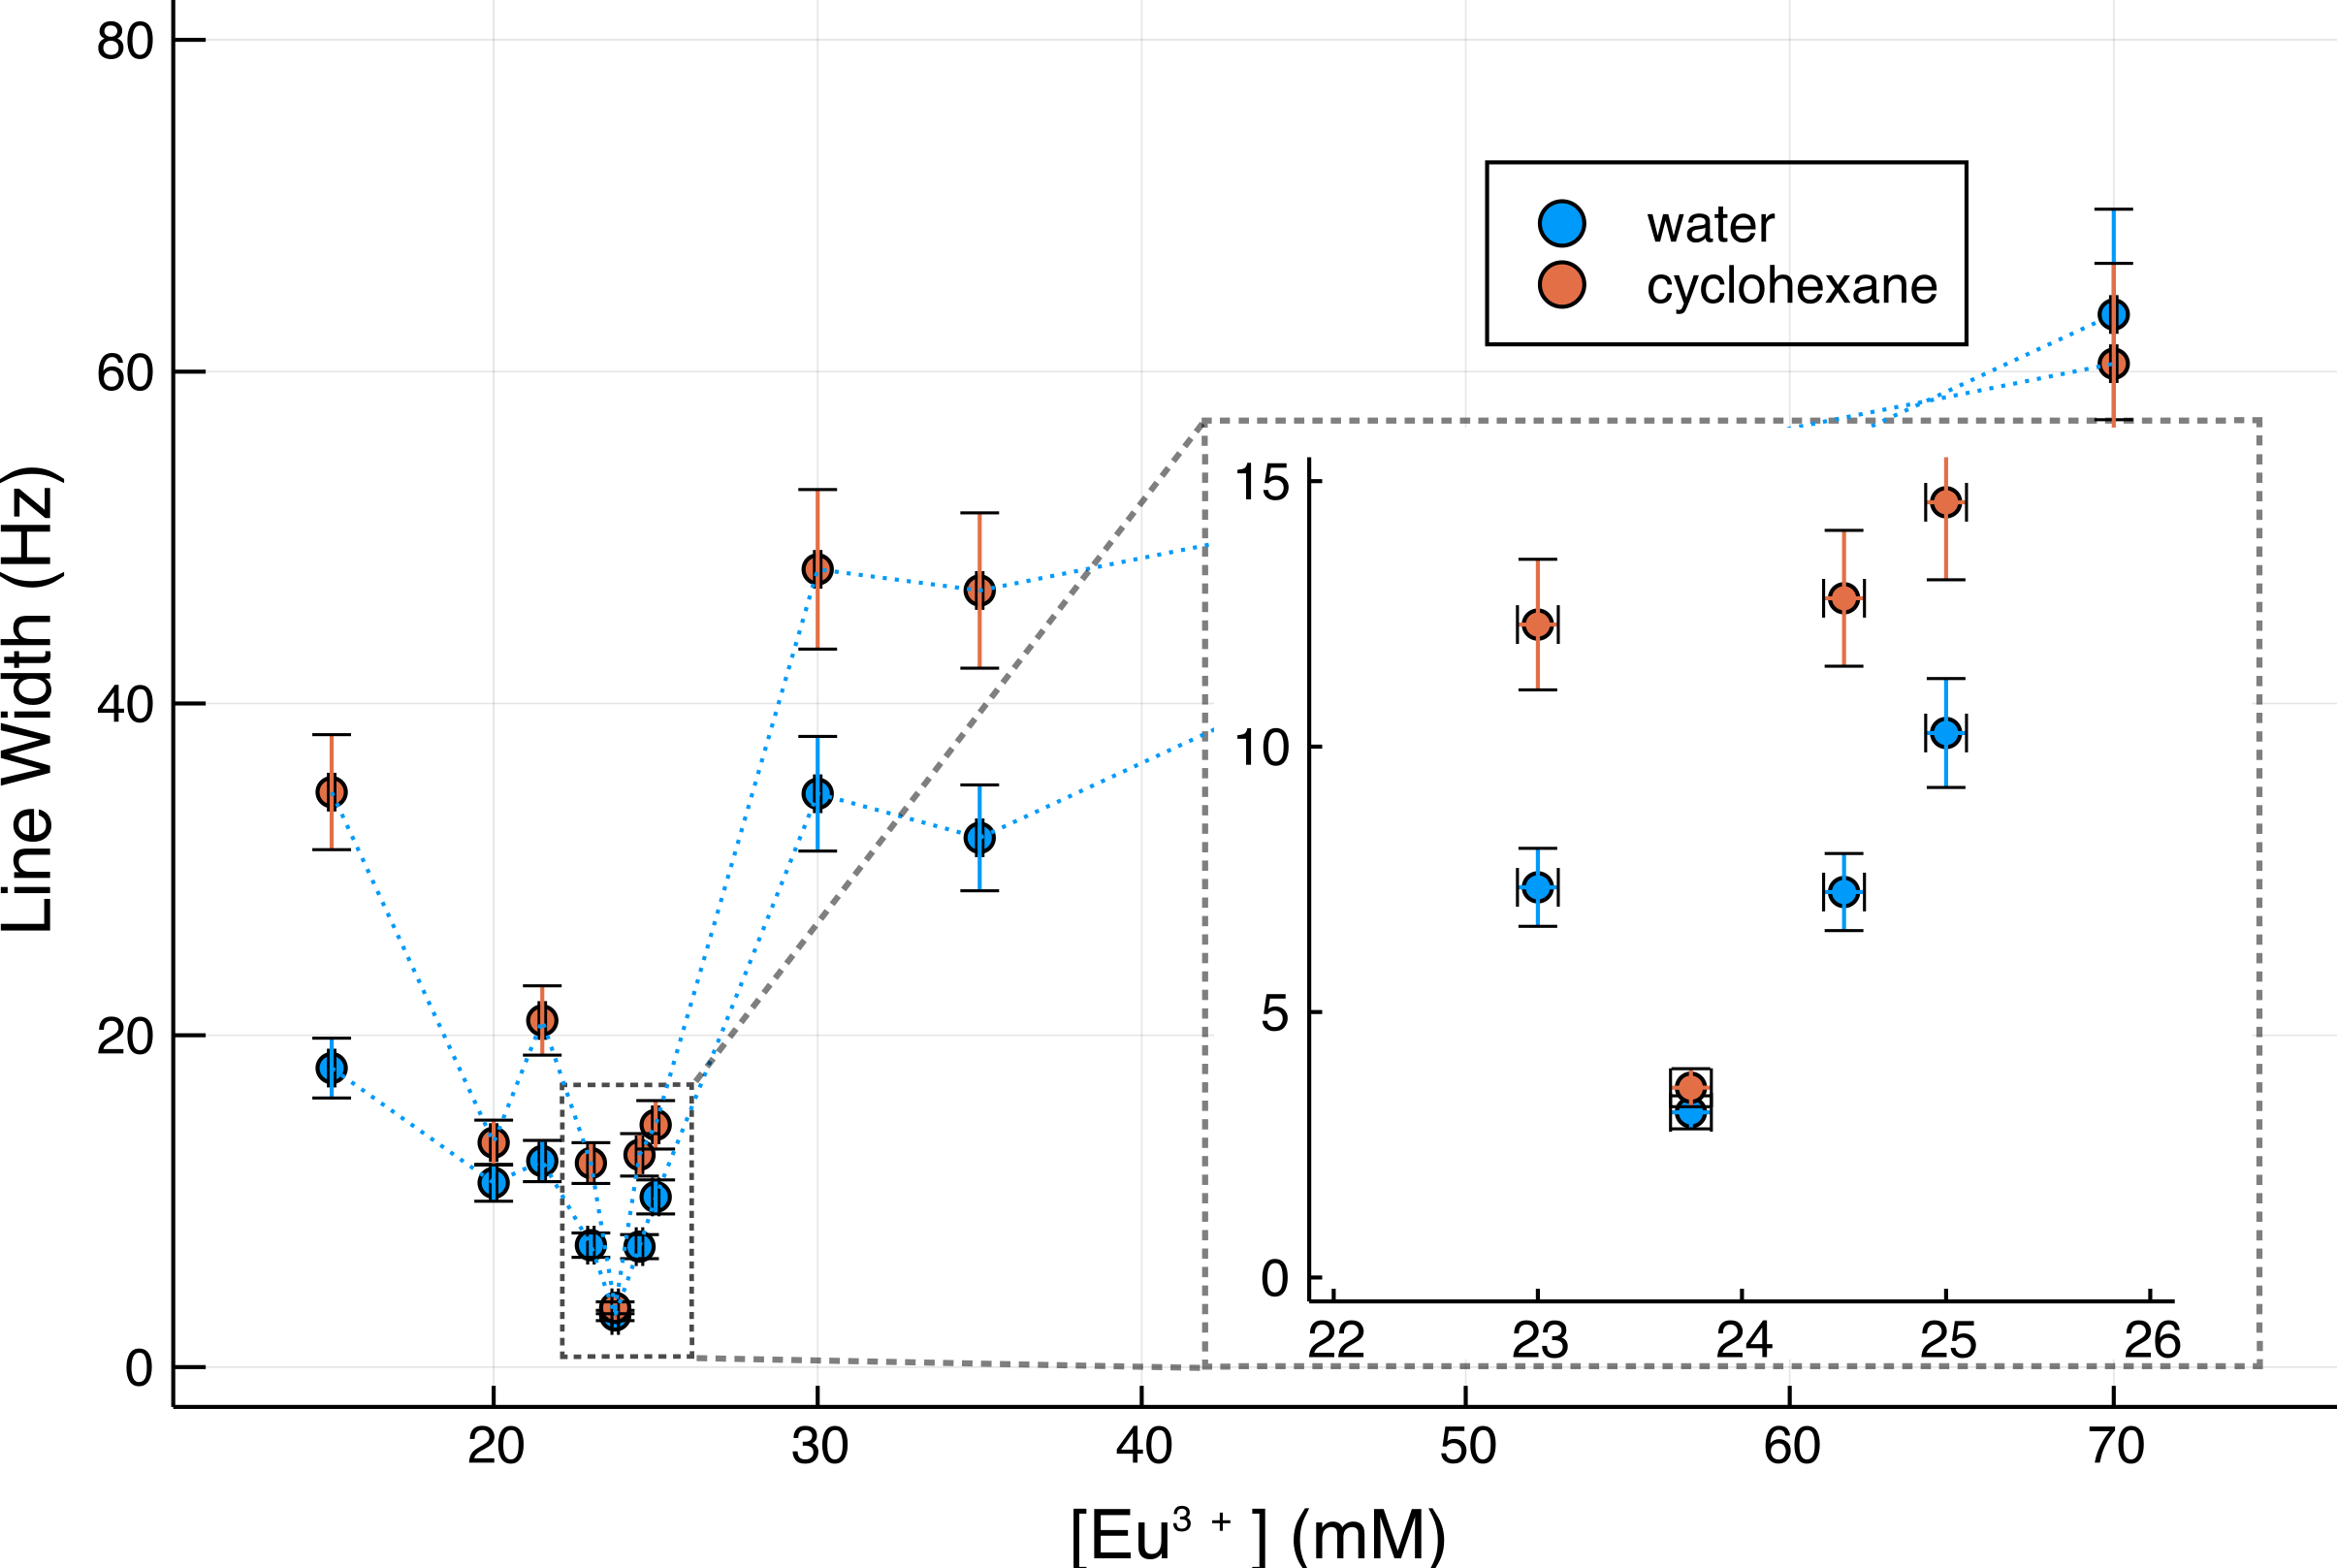
\includegraphics[width=0.8\columnwidth]{mu1y11-dnmr-fi-180618-droplet-lw-mod.png}
  \end{center}
  \caption{Observed line widths of water (blue circles) and
    cyclohexane (orange circles) in microfluidic droplet emulsions
    as a function of the $\ce{Eu[DTPA]^{2-}}$ concentration in the aqueous phase. Inset is the plot around the minimum
    concentration.
    The widths of both lines are minimal
    at the matched concentration of 23.75~mM. }
    \label{fig:linewidths}
\end{figure}


\begin{figure}
  \begin{center}
    \includegraphics[width=1.0\columnwidth]{Field-Maps.pdf}
  \end{center}
  \caption{$B_0$ Field maps obtained by magnetic resonance imaging of emulsions
  with (A) $\Delta\chi=-1.41\times 10^{-6}$ and (B) $\Delta\chi\approx 0$.
  }
  \label{fig:field-map}
\end{figure}




\section{Results and Discussion}


While it is possible to predict the magnetic field distribution in a system of
multiple phases with differing susceptibilities by solving the magnetostatic
equation, this requires precise geometric information on the arragement of the
two phases. In the case of an emulsion, the arrangement of the droplets is not
regular. However, at high droplet densities, it can be
expected to approximate  a dense packing of spheres. In order to obtain a
semi-quantitative prediction, the demagnetising field in
face-centred cubic  (FCC) and simple cubic (SC) lattices of diamagnetic spheres was simulated;
the results are shown in  \fig{fig:FEM-fcc}. A single unit cell containing
one (SC) or
two (FCC) independent spheres was meshed under periodic boundary conditions in all
directions (\fig{fig:FEM-fcc}C).
As is well known, the demagnetising field inside an isolated diamagnetic sphere
is homogeneous, while the field outside of the
sphere is that of a magnetic
point dipole located at the sphere's centre. This situation is approximated
in a lattice if the lattice constant is much larger than the sphere
diameter. The computed demagnetising field
of a small sphere in an SC lattice is shown in \fig{fig:FEM-fcc}A.
The contour levels display the $z$-component of the local demagnetising field
normalised by the background $B_0$ field and the susceptibility difference
$\Delta\chi= \chi_\text{sphere}-\chi_\text{continuous}$. The field is homogeneous
inside the sphere, and a spatially varying demagnetising field only
exists in the continuous phase.
By contrast, in a
densely packed face-centered cubic lattice the field is no
longer homogeneous inside the spheres (\fig{fig:FEM-fcc}B). The FCC
lattice approximates the geometry of a dense microemulsion of homogenous
water-in-oil droplets.  \fig{fig:FEM-fcc}D shows the histograms of
the $z$-components of
the demagnetisig field in the continuous and droplet phases of the FCC
lattice, respectively.

The NMR spectra expected from an ideal emulsion of the same geometry can
be predicted from these histograms
(neglecting no broadening contributions from the sample container).
The magnetic field relevant for nuclear Larmor precession, often referred
to as the "external" field\citep{Levitt:1996tg} $\mathbf{B}_\text{ext}$  is
given by\citep{Ryan:2014hl}

\begin{equation}
\mathbf{B}_\text{ext}(\mathbf{r})
= B_0 (1+\frac{\chi_s}{3}) \mathbf{e}_z  - {\mu_0} \nabla U_d(\mathbf{r}),
\end{equation}

where $B_0$ is the magnitude of the external field, $\chi_s$ is the local
magnetic susceptibility, and $U_d(\mathbf{r})$ is the scalar magnetic potential
of the demagnetising field. The volume susceptibility of a solution containing a
paramagnetic species at low concentration $c_p$ is
\begin{equation}
    \chi_s \approx \chi_0 + c_p\,\zeta_P,
\end{equation}
where $\chi_0$ is the volume susceptibility of the pure solvent,
and $\zeta_P$ is the
molar susceptibility of the paramagnetic species. $\zeta_P$ depends
slightly on the molecular environment. For example, values of
$5.86\cdot 10^{-5}\;\mathrm{l/\text{Mol}}$,
$5.68\cdot 10^{-5}\;\mathrm{l/\text{Mol}}$, and
$6.14\cdot 10^{-5}\;\mathrm{l/\text{Mol}}$ have been measured at 300K for
$\ce{Eu_2O_3}$, $\ce{EuF_3}$, and $\ce{EuBO_3}$, respectively\citep{Takikawa:2010iw}
To our knowledge, the precise molar susceptibility of $\ce{Eu[DTPA]^{2-}}$ in
aqueous solution has not been measured to date, but it is likely to be
similar to the above values.

\fig{fig:droplet-spectra} shows $^1$H NMR spectra obtained from emulsions in the chip
shown in \fig{fig:chip-design} with varying $\ce{Eu[DTPA]^{2-}}$ concentrations in the aqueous
phase as indicated in the figure. While the spectra are extremely broad without dopant,
concentrations in the vicinity of 23~mM lead to much sharper lines for both water and cyclohexane,
and the pure phase line widths are recovered at the optimum concentration of $c_p=23.75$~mM.
Using the susceptibilities given in
Table \ref{tab:suscept}, this leads to molar susceptibility for $\ce{Eu[DTPA]^{2-}}$
of $5.94\cdot 10^{-5}\;\mathrm{l/\text{Mol}}$, well within the range
 of molar susceptibilities reported in literature for other $\ce{Eu^{3+}}$
 compounds. Using this value, the histograms
shown in \fig{fig:FEM-fcc}D can be converted into
predicted emulsion NMR spectra as a function of $\ce{Eu[DTPA]^{2-}}$
concentration in the aqueous phase,
as shown in \fig{fig:predicted-spectra}.
The predicted behaviour is qualitatively similar to the experimental observation; very broad
lines are expected at zero dopant concentration, while sharp lines are recovered near the optimum
concentration. Also, the droplet phase peak is predicted to be narrower than the one from the continuous phase; this is already evident
in the histograms in \fig{fig:FEM-fcc}.  However, the predicted spectra are consistently sharper than the experimentally
observed ones.
It is not entirely clear what causes the discrepancy between the experimental observation
and the simulations. However, it should be noted that the experimental geometry of the emulsion
differs significantly from the simulation; the droplets are neither uniform in size, nor are they
arranged in a crystalline (FCC) lattice.


\begin{figure}
\begin{center}
	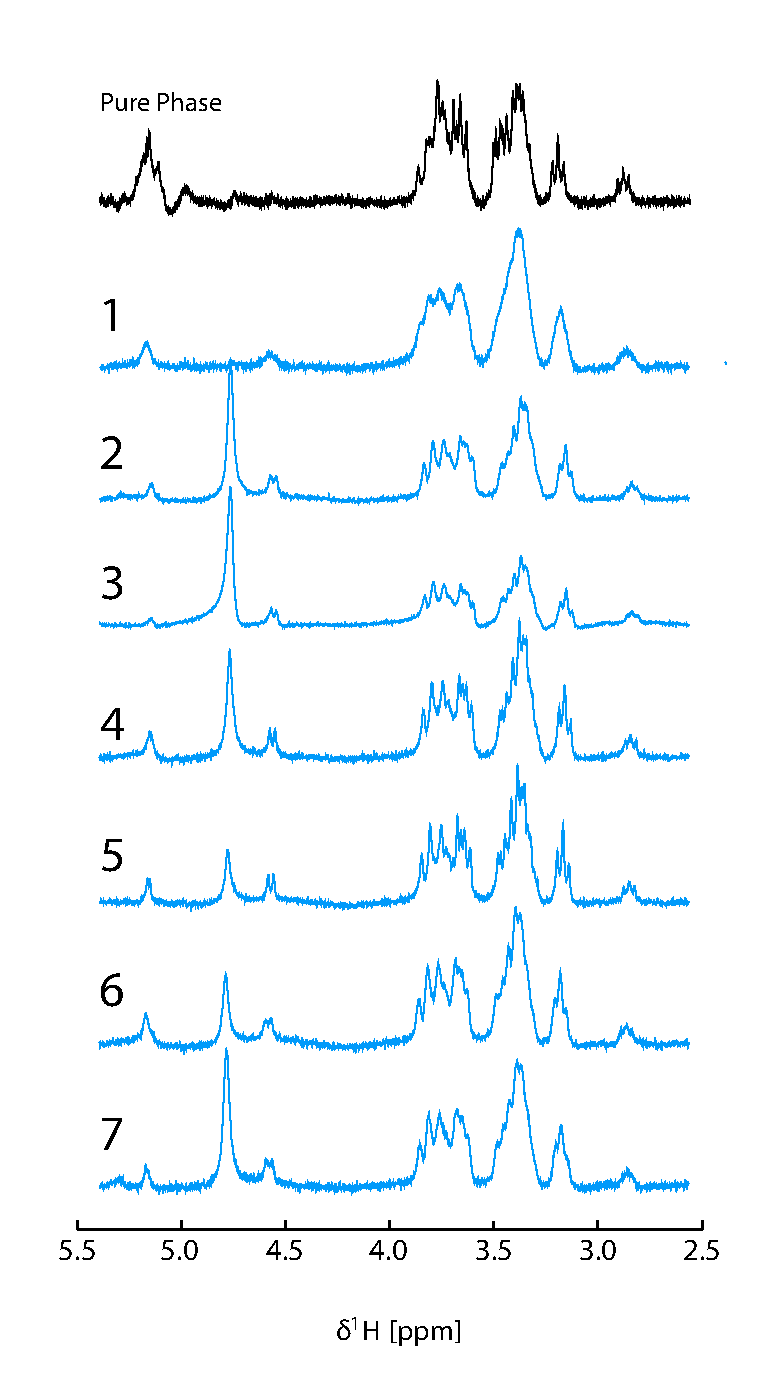
\includegraphics[width=0.7\columnwidth]{wgh2g11-dnmr-fi-180414-001-glucose-wsup}
\end{center}
\caption{Spectra of 200~mM Glucose in $\ce{H_2O}$ obtained from microfluidic droplet emulsions in
	cyclohexane. 1: Aqueous phase contains $c_0=23.75\pm0.25$~mM $\ce{Eu[DTPA]^{2-}}$. Spectra 2-7
	have been obtained by gradual dilution of the aqueous phase with small amounts of DI water.
	2: $\ln c/c0 = -0.5\%$; 3: $\ln c/c0 = -0.75\%$; $4: \ln c/c0 = -0.875\%$;
	$5: \ln c/c0 = -1.0\%$; $6: \ln c/c0 = -1.125\%$; $7: \ln c/c0 = -1.25\%$. A spectrum of pure phase 200mM glucose
	with optimised Eu doping in the same chip is included for comparison (black). The nonuniform peak at 4.8 ppm is due to carrier frequency drift during water suppression }
\label{fig:glucose-dilution}
\end{figure}


The observed widths of the NMR signals from cyclohexane and water
are summarised in \fig{fig:linewidths}. Here, we define the line width as
the ratio of the peak integral to the peak height, multiplied by $2/\pi$. In the
case of Lorentzian line shapes, this definition is equivalent to the full width at half height
(FWHM). However, the expected line shapes from the droplet emulsion are very different
from a Lorentzian (\fig{fig:FEM-fcc}D), such that using the FWHM would be misleading.

Both line widths exhibit a narrow
minimum at 23.75~mM $\ce{Eu[DTPA]^{2-}}$ in the aqueous phase. The water and
cyclohexane minimum peak widths are 3.1~Hz and 3.5~Hz, respectively. For comparison, the best resolution
that has been reached with the same NMR probe is 1.76~Hz for a homogeneous
solution of 150~mM sodium acetate in $\ce{H_2O}$.\citet{Finch:2016gv}

\fig{fig:field-map} shows magnetic field ($B_0$) maps of the sample chambers filled
with droplet emulsions.
In these experiments, two separate
images with different echo times are acquired. The phase difference in each pixel is therefore
proportional to the echo time difference and to the local magnetic field. The echo time difference is constant
therefore the colour denotes the phase acquired by each pixel and can be used to
inform on the homogeneity of the magnetic field in the sample.

In \fig{fig:field-map}A, the droplets do not contain any paramagnetic dopant. As a result, the
susceptibilities of the phases are unmatched, and strong local magnetic field differences
are visible in the images. By contrast, the droplets in \fig{fig:field-map}B are doped with 23.75~mM
$\ce{Eu[DTPA]^{2-}}$. As is clearly visible in the image, the local differences in the magnetic
fields are strongly attenuated in this case.

While the above results have demonstrated that optimal line widths can be minimised in $^1$H NMR
spectra of microfluidic emulsions by paramagnetic doping,
the question remains if this is sufficient to resolve homonuclear
$J$-couplings of a few Hz. This is required in order to do meaningful NMR spectroscopy,
particularly in the context of complex metabolic mixtures.
The top trace in \fig{fig:glucose-dilution} shows a spectrum of 200 mM glucose
and 23.75~mM $\ce{Eu[DTPA]^{2-}}$ in water. The water signal has been suppressed by pre-saturation.
In this case, the resolution is about 3~Hz; such that e.g., the triplet at 3.2~ppm (which corresponds
to the proton in the 2-position on the $\beta$-glucose anomer) is clearly resolved.

Spectrum 1 in \fig{fig:glucose-dilution} has been obtained from
droplet emulsions, starting form an aqueous stock solution prepared to a nominal concentration
of 23.75~mM in $\ce{Eu[DTPA]^{2-}}$ and 200 mM in glucose.
Initially, the resolution in this spectrum is quite poor, in spite of
the attempt to dope at the previously determined optimum concentration. Estimates predicted
the pipetting and weighing errors to add up to an uncertainty in the concentration of the
stock solution of $\pm 1\%$.
Assuming the stock solution was too concentrated, rather than too dilute, it was
then gradually diluted with small amounts of DI water corresponding
to a change in concentration much less than the experimental error in each step.
As can be seen in spectra 2-7, the resolution gradually increases, and matches
the pure phase spectrum at spectrum 5, before it deteriorates again.
In practice, high resolution spectra therefore require careful calibration of the dopant
concentration. It may not be practical to achieve this in one step by preparing the stock
solution, particularly if small volumes (around 10 ml or so) are used as in our
experiments. Rather, a gradual dilution as in \fig{fig:glucose-dilution} may be required
to calibrate the $\ce{Eu[DTPA]^{2-}}$ concentration for an accurate match of
the aqueous and carrier fluid susceptibilities. However, if such a match is established,
the resulting resolution is as good as that of the pure aqueous solution.

\section{Conclusion}

In Conclusion, susceptibility differences between the chip,
the aqueous phase, and the oil phase in a microfluidic droplet system can
be successfully mitigated by a combination of structural shimming and
doping of the less diamagnetic of the liquid phases with a europium compound.
The ultimate resolution achieved is only slightly inferior to what has been
demonstrated in homogeneous solutions on a microfluidic chip and is suitable for high
resolution NMR spectroscopy.
